\documentclass[10pt,a4paper]{article}

%% Language and font encodings
\usepackage[brazil]{babel}
\usepackage[utf8x]{inputenc}
\usepackage[T1]{fontenc}

%% Sets page size and margins
\usepackage[a4paper,top=3cm,bottom=2cm,left=3cm,right=3cm,marginparwidth=1.75cm]{geometry}

%% Useful packages
\usepackage{amsmath}
\usepackage{graphicx}
\usepackage[colorinlistoftodos]{todonotes}
\usepackage[colorlinks=true, allcolors=blue]{hyperref}

\title{IF687 - INTRODUÇÃO À MULTIMÍDIA}
\author{Hugo Falcão}

\begin{document}
\maketitle

\begin{figure}[h!]
\centering
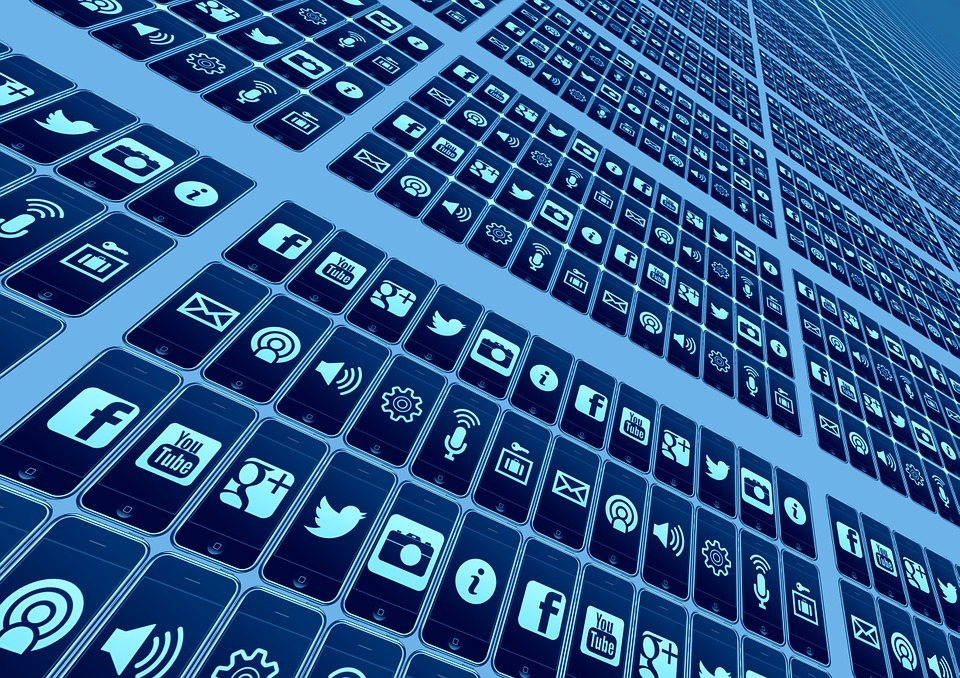
\includegraphics[width=0.5\textwidth]{Multimidia.jpg}
\caption{\label{fig:Multimidia}CC0 Creative Commons}
\end{figure}

%link da imagem: https://pixabay.com/pt/telefone-celular-smartphone-app-426559/
%licensa: CC0 Creative Commons

\section{Introdução}

A disciplina de Introdução à Multimídia foi introduzida ao currículo do CIn em resposta ao crescente interesse de alunos e docentes em se envolver com a área de desenvolvimento de plataformas e aplicações multimídia em geral. Por causa da escassez de material em português para estudo dessa área, tal cadeira supre uma necessidade muito vigente do mercado atual. Por sua matriz de assuntos, tal matéria pode ser encaixada dentro de Computação Gráfica, uma das grandes áreas da Computação.
\cite{siteCadeira}
    \\
    Dentre os tópicos principais acerca desta cadeira podemos encontrar as áreas de realidade virtual e realidade aumentada, interação com interfaces e interações sem-fio, ou até o estudo de unidades de processamento gráfico(GPU's).

\section{Relevância}
Esta cadeira tem uma imensa importância para um curso de Computação, isso porquê ela ensina fundamentos importantíssimos sobre como sobre gerir a implementação de mundos virtuais e sobre uma boa interação entre usuário e máquina, assim como um amplo entendimento de como tais mundos funcionam.

 \begin{enumerate}
 \item Desenvolve um conjunto de habilidades na área de mundos virtuais, com enfoque em entretenimento, arquiteturam educação, entre outros. 
 
 \item Apesar de assunstos muito interessantes, é possível que essa cadeira se proponha a ver assuntos demais para apenas uma cadeira. Isso pode acarretar em alunos com muitos conhecimentos, porém nenhum realmente aprofundado.
 
 \item Desperta o interesse em áreas de realidade virtual e realidade aumentada, que ainda tem significativo espaço no mercado atual.
 
 \end{enumerate}


\section{Relação com outras disciplinas}

\begin{table}[h!]
\centering
\label{my-label}
\begin{tabular}{|l|l|}
\hline
IF755 - REALIDADE VIRTUAL      & \begin{tabular}[c]{@{}l@{}}A disciplina de introdução à multimídia desen-\\ volve a capacidade do aluno a criar ambientes\\ de realidade virtual que são de grande impor-\\ tância para o mercado.\cite{VRIntro} \end{tabular}                                                                                                                                          \\ \hline
IF669 - INTRODUÇÃO À COMPUTAÇÃO & \begin{tabular}[c]{@{}l@{}}A disciplina de introdução à computação é uma\\ das cadeiras mais básicas do curso à medida que\\ ela desenvolve noções gerais de programação, \\ como a forma de pensar de um computeiro que \\ é indispensável para qualquer atuante da área.\end{tabular}                                                                  \\ \hline
IF680 - PROCESSAMENTO GRÁFICO   & \begin{tabular}[c]{@{}l@{}}A cadeira de processamento gráfico é de grande\\ importância para o curso de introdução à multi-\\ mídia visto que ela desenvolve habilidades im-\\ portantíssimas como a visualização espacial em\\ 3D.\end{tabular}                                                                                                         \\ \hline
IF794 - JOGOS AVANÇADOS         & \begin{tabular}[c]{@{}l@{}}A disciplina de Jogos avançados também tem \\ uma visível relação com a de introdução à multi-\\ mídia visto que ajuda, entre outras coisas, a de-\\ senvolver a capacidade de interação com ambi-\\ entes tridimensionais, assim como a entender a\\ necessidade de uma boa relação entre usuário e \\ máquina.\end{tabular} \\ \hline
\end{tabular}
\end{table}



\nocite{AR101}
\nocite{ARWiki}

\bibliographystyle{plain}
\bibliography{hsrf}

\end{document}